% Created 2021-03-08 Mon 10:20
% Intended LaTeX compiler: pdflatex
\documentclass[11pt]{article}
\usepackage[utf8]{inputenc}
\usepackage[T1]{fontenc}
\usepackage{graphicx}
\usepackage{grffile}
\usepackage{longtable}
\usepackage{wrapfig}
\usepackage{rotating}
\usepackage[normalem]{ulem}
\usepackage{amsmath}
\usepackage{textcomp}
\usepackage{amssymb}
\usepackage{capt-of}
\usepackage{hyperref}
\author{Sam Barrett}
\date{\today}
\title{Log Week 5}
\hypersetup{
 pdfauthor={Sam Barrett},
 pdftitle={Log Week 5},
 pdfkeywords={},
 pdfsubject={},
 pdfcreator={Emacs 27.1 (Org mode 9.5)}, 
 pdflang={English}}
\begin{document}

\maketitle
This week I first focused on implementing a macro-level route planner. To do this I used existing graphing libraries to encapsulate \texttt{Road} structure data as edges, with nodes being intersections or junctions. I then used Dikstra's algorithm to find shortest paths between a given set of starting and terminating positions. I was able to work out when two paths occupied the same stretch of road, and complete a cooperative plan for such sections. E.g. (1 -> 2 -> 3 -> 5) and (4 -> 2 -> 3 -> 1), may share the road between node 2 and 3 if \texttt{len(1 -> 2) + len(2 -> 3) < len(4 -> 2)} or \texttt{len(4 -> 2) + len(2 -> 3) < len(1 -> 2)}.

I went on to write benchmarking code and collect some results, I encountered some issues where the plotting library for Julia has some errors colouring 3D surfaces based on a 4th vector, but preliminary results look like:

\begin{center}
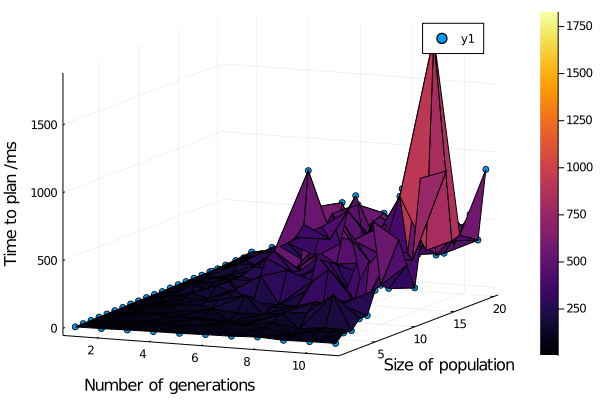
\includegraphics[width=.9\linewidth]{../../code/julia/images/single-agent-result.png}
\end{center}


I am intending for the colouring of the surface to be determined by the fitness of the individual at that point. Allowing me to see the effect of number of generations and size of population on both planning time and fitness of produced solutions.
\end{document}
